\section{Logaritmi}

\subsection{links}

\href{https://www.examsolutions.net/tutorials/exam-questions-logarithms/}{examsolutions.net}\footnote{\texttt{https://www.examsolutions.net/tutorials/exam-questions-logarithms/}}
, \href{https://www.studocu.com/it/document/liceo-scientifico-vito-volterra-fabriano-ancona/chimica-dei-materiali/3-log-l10-logaritmi/45324577}{studocu.com} \footnote{\texttt{https://www.studocu.com/it/document/liceo-scientifico-vito-volterra-fabriano-ancona} 

\texttt{/chimica-dei-materiali/3-log-l10-logaritmi/45324577}}
, \href{https://assets.cambridge.org/97811076/53153/excerpt/9781107653153\_excerpt.pdf}{cambridge.org}\footnote{\texttt{https://assets.cambridge.org/97811076/53153/excerpt/9781107653153\_excerpt.pdf}}
, \href{https://www.physicsandmathstutor.com/pdf-pages/?pdf=https\%3A\%2F\%2Fpmt.physicsandmathstutor.com\%2Fdownload\%2FMaths\%2FA-level\%2FC3\%2FSolutionbank-Edexcel\%2FChapter-5\%2FP3\%2520Exercise\%25205C.pdf}{physicsandmathstutor.com}\footnote{\texttt{https://www.physicsandmathstutor.com/pdf-pages/?pdf=https\%3A\%2F\%2Fpmt.}

\texttt{physicsandmathstutor.com\%2Fdownload\%2FMaths\%2FA-level\%2FC3\%2FSolutionbank-}

\texttt{Edexcel\%2FChapter-5\%2FP3\%2520Exercise\%25205C.pdf}}


\subsection{Definizione}

Il logaritmo è la funzione inversa dell'elevamento a potenza.

\textbf{Definizione di logaritmo}:

\[
\begin{split}
\log_a(b)&=x \\
\Rightarrow
a^x&=b
\end{split}
\]

Per tutti gli $x$, $y$ e $a$ $ \in \mathbb{R}, x>0$ e $a \neq 1$:

Esempio:

\[
\begin{split}
\log_2(8)&=3 \\
\\
\Rightarrow 2^3&=8
\end{split}
\]

Il grafico del logaritmo con base maggiore di 1 cresce sempre:

\begin{figure}[H]
\centering
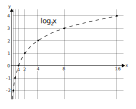
\includegraphics[width=0.7\textwidth]{log2x.pdf}
\end{figure}

Il grafico di $\log_2x$ attraversa l'asse $x$ a $x = 1$ e passa per i punti $(2, 1)$, $(4, 2)$, e $(8, 3)$

La curva si avvicina arbitrariamente all'asse $y$  senza toccarlo mai.

Per le basi minori di 1, il grafico decresce sempre:

\begin{figure}[H]
\centering
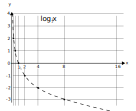
\includegraphics[width=0.7\textwidth]{log12x.pdf}
\end{figure}



\subsection{Ripassino formule sulle potenze}

\begin{enumerate}
\item $a^m \cdot a^n = a^{m+n}$
\item $\frac{a^m}{a^n}=a^{m-n}$
\item $(a^m)^n=a^{m\cdot n}$
\item $a^\frac{m}{n}=\sqrt[n]{a^m}$
\item $a^{-n}=\frac{1}{a^n}$
\item $a^n \cdot b^m=(ab)^n$
\item $\frac{a^n}{b^n}=\left(\frac{a}{b}\right)^n$
\end{enumerate}


\subsection{Relazioni e proprietà dei logaritmi}

\begin{minipage}{\textwidth}
\begin{enumerate}

\item Prodotto $\Leftrightarrow$ somma:
\[
\log_a(x\cdot y)=log_a(x) + log_a(y)
\]

\item Quoziente $\Leftrightarrow$ differenza:
\[
\log_a\left(\frac{x}{y}\right)=log_a(x) - log_a(y)
\]

\item Potenza:
\[
\log_a\left(x^y\right)=y \cdot log_a(x)
\]

\item Radice:
\[
\log_a\left(\sqrt[p]{x}\right)=\frac{log_ax}{p}
\]

\item Cambiamento di base:
\[
\log_ax=\frac{log_kx}{log_ka}\textrm{ per qualsiasi }k
\]


\item 
\[
\log_a1=0\textrm{ per tutti gli }a>0\textrm{ e }a\neq 1
\]



\item 
\[
\log_aa=1\textrm{ per tutti gli }a>0\textrm{ e }a\neq 1
\]


\item 
\[
a^{\log_ab}=b
\]


\end{enumerate}

\end{minipage}

\subsection{Cosa \textbf{NON} si può fare con i logaritmi}

\begin{enumerate}
\item $\log(x + y)$ rimane così; \textbf{NON} si può semplificare in $log x + log y$
\item $\log(e^x+e^y)$ rimane così;\textbf{NON} non si può semplificare in $x + y$
\item $(\log(x))^2$ \textbf{NON} è $2\log(x)$; la formula giusta è $\log(x^2)=2\log(x)$
\item $a^{2+\log(x)}=a^2a^{log(x)}$ \textbf{NON} $a^2+x$
\end{enumerate}

\subsection{Esercizi}
\subsubsection{Valori numerici}\label{subsec:val_num}

\begin{enumerate} % ese_numeri
\item  
\[
2\log_{12}3+4\log_{12}2=\ldots
\]
\rightline{( Soluzione a pagina \pageref{soln_1} \label{exn_1}\label{exn_1} )}


\item \[
\log_825+\log_810-3\log_85=\ldots
\]

\item \[
2\log_{10}20-(\log_{10}5+\log_{10}8)=\ldots
\]

\item \[
4\log_32-\log_34-2\log_3\sqrt{3}-\log_312=\ldots
\]

\item \[
4\cdot\log_2\left(\frac{1}{4}\right)-3\cdot\log_{\frac{1}{2}}(32)=\ldots
\]

\item\[
\frac{1}{2}\log_{\frac{2}{3}}\left(\frac{4}{9}\right)
-2\log\frac{2}{3}\left(\frac{9}{4}\right)=\ldots
\]

\end{enumerate} % ese_numeri

\subsubsection{Equazioni}\label{subsec:equazioni}

\begin{enumerate}[label={Esercizio \arabic* },wide = 1cm, font =\bfseries]

\item 
\[
\log_2\left(\frac{5}{4}x-1\right)=-2
\]
\rightline{( Soluzione a pagina \pageref{sol_1} \label{ex_1}\label{ex_1} )}

\item 
\[
\log_2\frac{2x}{x+3}=-1
\]
\rightline{( Soluzione a pagina \pageref{sol_2}\label{ex_2} )}

\item 
\[
\log_2(w^2+4w+3)=4+\log_2(w^2+w)
\]
\rightline{( Soluzione a pagina \pageref{sol_3} \label{ex_3}\label{ex_3} )}

\item \[
\log_38-3\cdot\log_3t=3
\]

\item \[
2\log_3 x-log_3(x-2)=2
\]


\item Sapendo che \[
y=3\cdot x^2
\]

verificare che \[
\log_3 y = 1 + 2\log_3 x
\]

\item \[
1+2\log_3 x = \log_3 (28x -9)
\]


\item \[
5^{(2x)}-12\cdot 5^x + 35 = 0
\]

\item \[
7^{2x}-4\cdot 7^x+3=0
\]


\item\[
\frac{
\log_232+\log_216
}{
\log_2x
}=\log_2x
\]

\item Sapendo che $a$ e $b$ sono positivi, risolvere

\[
\left\{
\begin{array}{ll}
a = 3b\\
\log_3 a + \log_3 b = 2
\end{array}
\right.
\]


\item \[
\log_2(11-6x) = 2\cdot \log_2(x-1)+3
\]

\item \[
2\log_2(x+15)-\log_2x=6
\]



\end{enumerate}


\subsubsection{Multiple Choice}\label{subsec:mult_choice}

Soluzioni a pagina \pageref{sol_mc} \label{ex_mc}\label{ex_mc}

\begin{enumerate}

\item Per $a>0$ e $a\neq 1$ quale delle seguenti affermazioni è corretta?

\begin{choices}
\choice Se $M=N$ allora $\log_aM=\log_aN$
\choice Se $\log_aM=\log_aN$ allora $M=N$
\choice Se $\log_aM^2=\log_aN^2$ allora $M=N$
\choice Se $M=N$ allora $\log_aM^2=\log_aN^2$
\end{choices}

\item Se $\log_ab=c$, allora \ldots

\begin{choices}
\choice $a^c=b$
\choice $a^b=c$
\choice $c^a-b$
\choice $c^b=a$
\end{choices}

\item Il dominio del numero reale $a$ nella formula $b=\log_{a-2}(5-a)$ è \ldots

\begin{choices}
\choice $(-\infty, 5)$
\choice $(2, 5)$
\choice $(2, 3)\cup(3, 5)$
\choice $(2, +\infty)$
\end{choices}

\item Data l'equazione
\[
\left(\frac{1}{2}\right)^3=\frac{1}{8}
\]

Quale delle seguenti affermazioni è corretta?


\begin{choices}
\choice $\log_{\frac{1}{2}}3=\frac{1}{8}$
\choice $\log_{\frac{1}{2}}\frac{1}{8}=3$
\choice $\log_{\frac{1}{8}}\frac{1}{2}=3$
\choice $\log_3\frac{1}{2}=\frac{1}{8}$
\end{choices}

\item Qual'è il valore della seguente espressione?

\[
3^{2+\frac{1}{2}\log_32}
\]

\begin{choices}
\choice $9+\sqrt{2}$
\choice $9+\frac{\sqrt{2}}{2}$
\choice $9\sqrt{2}$
\choice $10$
\end{choices}

\end{enumerate}

\subsubsection{Completare le espressioni date}\label{subsec:compl_espr}


\begin{enumerate}
\item \[
\log_3(2x-1)=1\textrm{, }x=\ldots?
\]


\item 
\[ % completare
ln(lg 10)+ \sqrt{(\pi -4)^2}=\ldots?
\]
\rightline{( Soluzione a pagina \pageref{sol_4_5} \label{ex_4_5}\label{ex_4_5} )}


\item 
Data la seguente funzione:

\[
f(3x)=\log_2{\sqrt{\frac{9x+1}{2}}}
\]

Quanto vale $f(1)$?

\rightline{( Soluzione a pagina \pageref{sol_5} \label{ex_5}\label{ex_5} )}

\end{enumerate}

\subsubsection{Domanda e risposta}\label{subsec:dom_risp}


\begin{enumerate}
\item
\[
\log_5(log_3x)=0\textrm{, }x=\ldots?
\]

\item
\[
\log_3(lg x)=1\textrm{, }x=\ldots?
\]

\item
\[
lg[\log_2(lg x)]=0\textrm{, }x=\ldots?
\]

\item

Trovare il valore di $\frac{x^2}{y}$ sapendo che 

\[
\left\{
\begin{array}{ll}
\log_\frac{1}{2} x=m\\
\log_{\frac{1}{4}}y=m+2
\end{array}
\right.
\]

\rightline{( Soluzione a pagina \pageref{sol_6} \label{ex_6}\label{ex_6} )}

\item

\[
\log_3(x+1)=3-log_3(x+7)
\]

\rightline{( Soluzione a pagina \pageref{sol_7} \label{ex_7}\label{ex_7} )}

\item

\[
\log(x^2)=(log(x))^2 
\]

\rightline{( Soluzione a pagina \pageref{sol_8} \label{ex_8}\label{ex_8} )}


\item
\[
\log(x-1)-log(x+1)=log(x-3)-log(x-2)
\]

\rightline{( Soluzione a pagina \pageref{sol_9} \label{ex_9}\label{ex_9} )}


\item Trovare $x$ per 

\[
4\cdot 5^{x+1} = 3^x
\]

\rightline{( Soluzione a pagina \pageref{sol_10} \label{ex_10}\label{ex_10} )}

\item 
\[
5^{3x+1}=15
\]

\item 
\[
3^{2x+1}=4^{x-2}
\]

\item 
\[
3\cdot 2^{x-3}=\frac{1}{5^{2x}}
\]


\item 
\[
3^{2x+1}-11\cdot 3^x=4
\]

\rightline{( Soluzione a pagina \pageref{sol_11} \label{ex_11}\label{ex_11} )}

\item
\[
2^{2x}-5 \cdot 2^x + 4 = 0
\]

\item
\[
e^x-6\cdot e^{-x}=5
\]

\item
\[
\left\{
\begin{array}{ll}
e^{x+y}=6\\
e^x+e^y=5
\end{array}
\right.
\]

\item 

Date le relazioni:

\begin{itemize}
\item $x = \log a$
\item $y = \log b$
\item $z = \log c$
\end{itemize}

Scrivere $2x+y-\frac{1}{2}z+2$ come un singolo logaritmo $\log(W)$.

\rightline{( Soluzione a pagina \pageref{sol_12} \label{ex_12}\label{ex_12} )}

\item

\[
\left\{
\begin{array}{ll}
x = \log a \\
y = \log b \\
z = \log c
\end{array}
\right.
\]

scrivere $2x + y - 0.5z + 2$ come un singolo logaritmo.

\item 

\[
\left\{
\begin{array}{ll}
a = \log x \\
b = \log y \\
c = \log z
\end{array}
\right.
\]

Trovare $a$, $b$ e $c$ per

\[
\log\left(
\frac{
10xy^2
}{
\sqrt{z}
}
\right)
\]

\item $ $

Sapendo che $\log a + 1 = \log b^2$, scrivere $a$ in termini di $b$

\item $ $

Sapendo che $\ln y = 2 + 4 \ln x$, scrivere $y$ in termini di $x$

\item $ $

Date le equazioni

\[
\left\{
\begin{array}{ll}
e^{2x}+e^y=800\\
3\ln x+\ln y = 5
\end{array}
\right.
\]

Per ognuna delle due equazioni esprimere $y$ in termini di $x$.

Dopodiché risolvere il sistema.

\item 
\[
4\log_4 x=9\log_x 4
\]
\rightline{( Soluzione a pagina \pageref{sol_13} \label{ex_13}\label{ex_13} )}

\item \[
\log_4x+\log_4(x-6)=2
\]

\item \[
2\log_2 x-\log_2(x+1)=3
\]

\item \[
25\log_2x=\log_x2
\]

\item \[
\log_4(4-x)\log_{16}(9x^2-10x+1)
\]

\end{enumerate}

\subsubsection{Applicazioni dei logaritmi in Fisica}\label{subsec:val_num}

\begin{enumerate}

\item{\ }

\begin{center}
\fbox{\begin{minipage}{0.9\textwidth}
When a cup of tea is made, its temperature is $85^\circ$C.

After 3 minutes the tea has cooled to $60^\circ$C.

That the temperature $T(^\circ C)$ of the cup of tea decays exponentially according to the function
\[
T = A + Ce^{-0.2t}
\]
, where $t$ is the time measured in minutes.

Find:\begin{itemize}
\item the values of $A$ and $C$
\item the time it takes for the tea to cool to $40^\circ$C.
\end{itemize}

\end{minipage}}
\end{center}
\rightline{( Soluzione a pagina \pageref{solf_1} \label{exf_1}\label{exf_1} )}

\item{\ }

\begin{center}
\fbox{\begin{minipage}{0.9\textwidth}
The amount of reactant, $V$ (grams), in a chemical reaction decays exponentially according to the function

\[
V = M + Ce^{-0.32t}
\]

where $t$ is the time in seconds since the start of the reaction.

Initially there was $4.5 g$ of reactant, and this had decayed to $2.6 g$ after $7$ seconds.

Find:\begin{itemize}
\item the values of $C$
\item the value that the amount of reactant approaches in the long term.
\end{itemize}

\end{minipage}}
\end{center}

\vspace{0.5cm}

\item{\ }

\begin{center}
\fbox{\begin{minipage}{0.9\textwidth}
A population of bacteria grows according to the model 

\[
P = Ae^{kt}
\]

where $P$ is the size of the population after $t$ minutes.

Given that after $2$ minutes there are $200$ bacteria and after $5$ minutes there are $1500$ bacteria, find the size of the population after 10 minutes.

\end{minipage}}
\end{center}

\end{enumerate}


\subsubsection{Problemi misti}\label{subsec:prob_mix}

\begin{enumerate}
\item Risolvere 
\[
3\cdot 9^x -10\cdot 3^x + 3 = 0
\]
\item Risolvere 
\[
2^{3x+1}=5^{5-x}
\]
\item Risolvere 
\[
\left\{
\begin{array}{ll}
\ln x^2 + \ln y =15\\
\ln x + \ln y^3 = 10
\end{array}
\right.
\]
\item Esprimere $x$ in termini di $y$:
\[
y=\ln x-\ln(x+2)+\ln(x^2-4)\\
\]
\item La curva $y=4\ln(x-a)$ passa per il punto $(5, \ln 16)$; trovare a
\item
\begin{enumerate}
\item 
An economic model predicts that the demand $D$, for a new product will grow according to the equation

\[
D = A - Ce^{-0.2t}
\]
where $t$ is the number of days since the product launch.
After 10 days the demand is 15,000 and it is increasing at a rate of 325 per day.

\begin{enumerate}
\item Find the value of $C$.
\item Find the initial demand for the product.
\item Find the long-term demand predicted by this model.
\end{enumerate}
\item  An alternative model is proposed, in which the demand grows according to the formula

\[
D=B\ln\left(
\frac{
t+10
}{
5
}
\right)
\]
The initial demand is the same as that for the first model.

\begin{enumerate}
\item Find the value of $B$.
\item What is the long-term prediction of this model?
\end{enumerate}

\item After how many days will the demand predicted by the second model become larger than the demand predicted by the first model?

\end{enumerate}
\end{enumerate}

\subsubsection{Esercizi Difficili}\label{subsec:eser_diff} %esercizi

\begin{enumerate} % esercizi difficili
\item Trovare la soluzione di % esercizi difficili
\[
2^{3x-4}\cdot3^{2x-5}=36^{x-2}
\]
scritta come $\frac{\ln p}{\ln q}$ dove $p$ e $q$ sono interi.
\item Date le espressioni % esercizi difficili
\[
\log_a b^2=c^2
\]

\[
\log_b a = c+1
\]
esprimere $a$ in termini di $b$.
\item  % esercizi difficili
In a physics experiment, the technician measured how the force $F$ exerted by a spring depends on its extension $x$.

She then plotted the values of $a = \ln F$ and $b = \ln x$ on a graph, with $b$ on the horizontal axis and $a$ on the vertical axis.

The graph was a straight line, passing through the points $(2, 4.5)$ and $(4, 7.2)$.

Find an expression for $F$ in terms of $x$.

\item Math Olympiad question!  

\[
25^x-15^x=9^x
\]
\rightline{( Soluzione a pagina \pageref{solf_2} \label{exf_2}\label{exf_2} )}


\item 

\[
100^{\left(\frac{1}{2}\lg9-lg2\right)}-\log_98\cdot\log_4\sqrt[3]{3}
\]

\rightline{( Soluzione a pagina \pageref{solf_3} \label{exf_3}\label{exf_3} )}


\end{enumerate} % esercizi difficili


